\graphicspath{{Img/regrasping/}}

\section{Regrasping a rope}

    \subsection{Assignment}
        The last use case concerns regrasping a piece of a rope from one gripper to the other.

        The proposed scenario is the following.  It starts with the left gripper holding one end of the rope. The right gripper is open and is positioned towards the left gripper (see Figure~\ref{fig:RegraspInit}).
%
        \begin{enumerate}\itemsep0pt
            \item The left arm starts to move towards the right gripper.
            \item When the presence of the rope is detected inside the right gripper, the motion of the left arm is stopped.
            \item The right gripper closes, thus holding the other end of the rope.
            \item The left gripper opens and releases the rope.
            \item The left arm moves back and the functions of both arms are swapped.
            \item The whole procedure is repeated again. The right arm now moves towards the left one that catches the rope.
        \end{enumerate}

        \begin{figure}[h]
        \includegraphics[width=0.5\textwidth]{RegraspInit.png}
        \centering
        \caption{The initial position for regrasping the rope.}
        \label{fig:RegraspInit}
        \end{figure}

    \subsection{Regrasping workflow}
        In the following text, I use the definition of points shown in Figure~\ref{fig:GraspPoses} (front view). Points $P_{a,b,c}$ are connected with the left arm, while points $P_{1,2,3}$ are connected with the right arm. Point $P_0$ is used as the default point from which the rest of the points is calculated using the parameters $l$ and $h$, $l$ denotes the distance between the grippers and $h$ the length of the rope.

        \begin{figure}[h]
        \includegraphics[width=0.5\textwidth]{GraspPoses.pdf}
        \centering
        \caption{Defining the points.}
        \label{fig:GraspPoses}
        \end{figure}

        Based on the assignment, I designed the rope regrasping workflow that is shown in Figure~\ref{fig:RegraspingWorkflow}. The states of the procedure are shown in Figure~\ref{fig:RegraspingProcedure} and are described below.

        \begin{figure}
        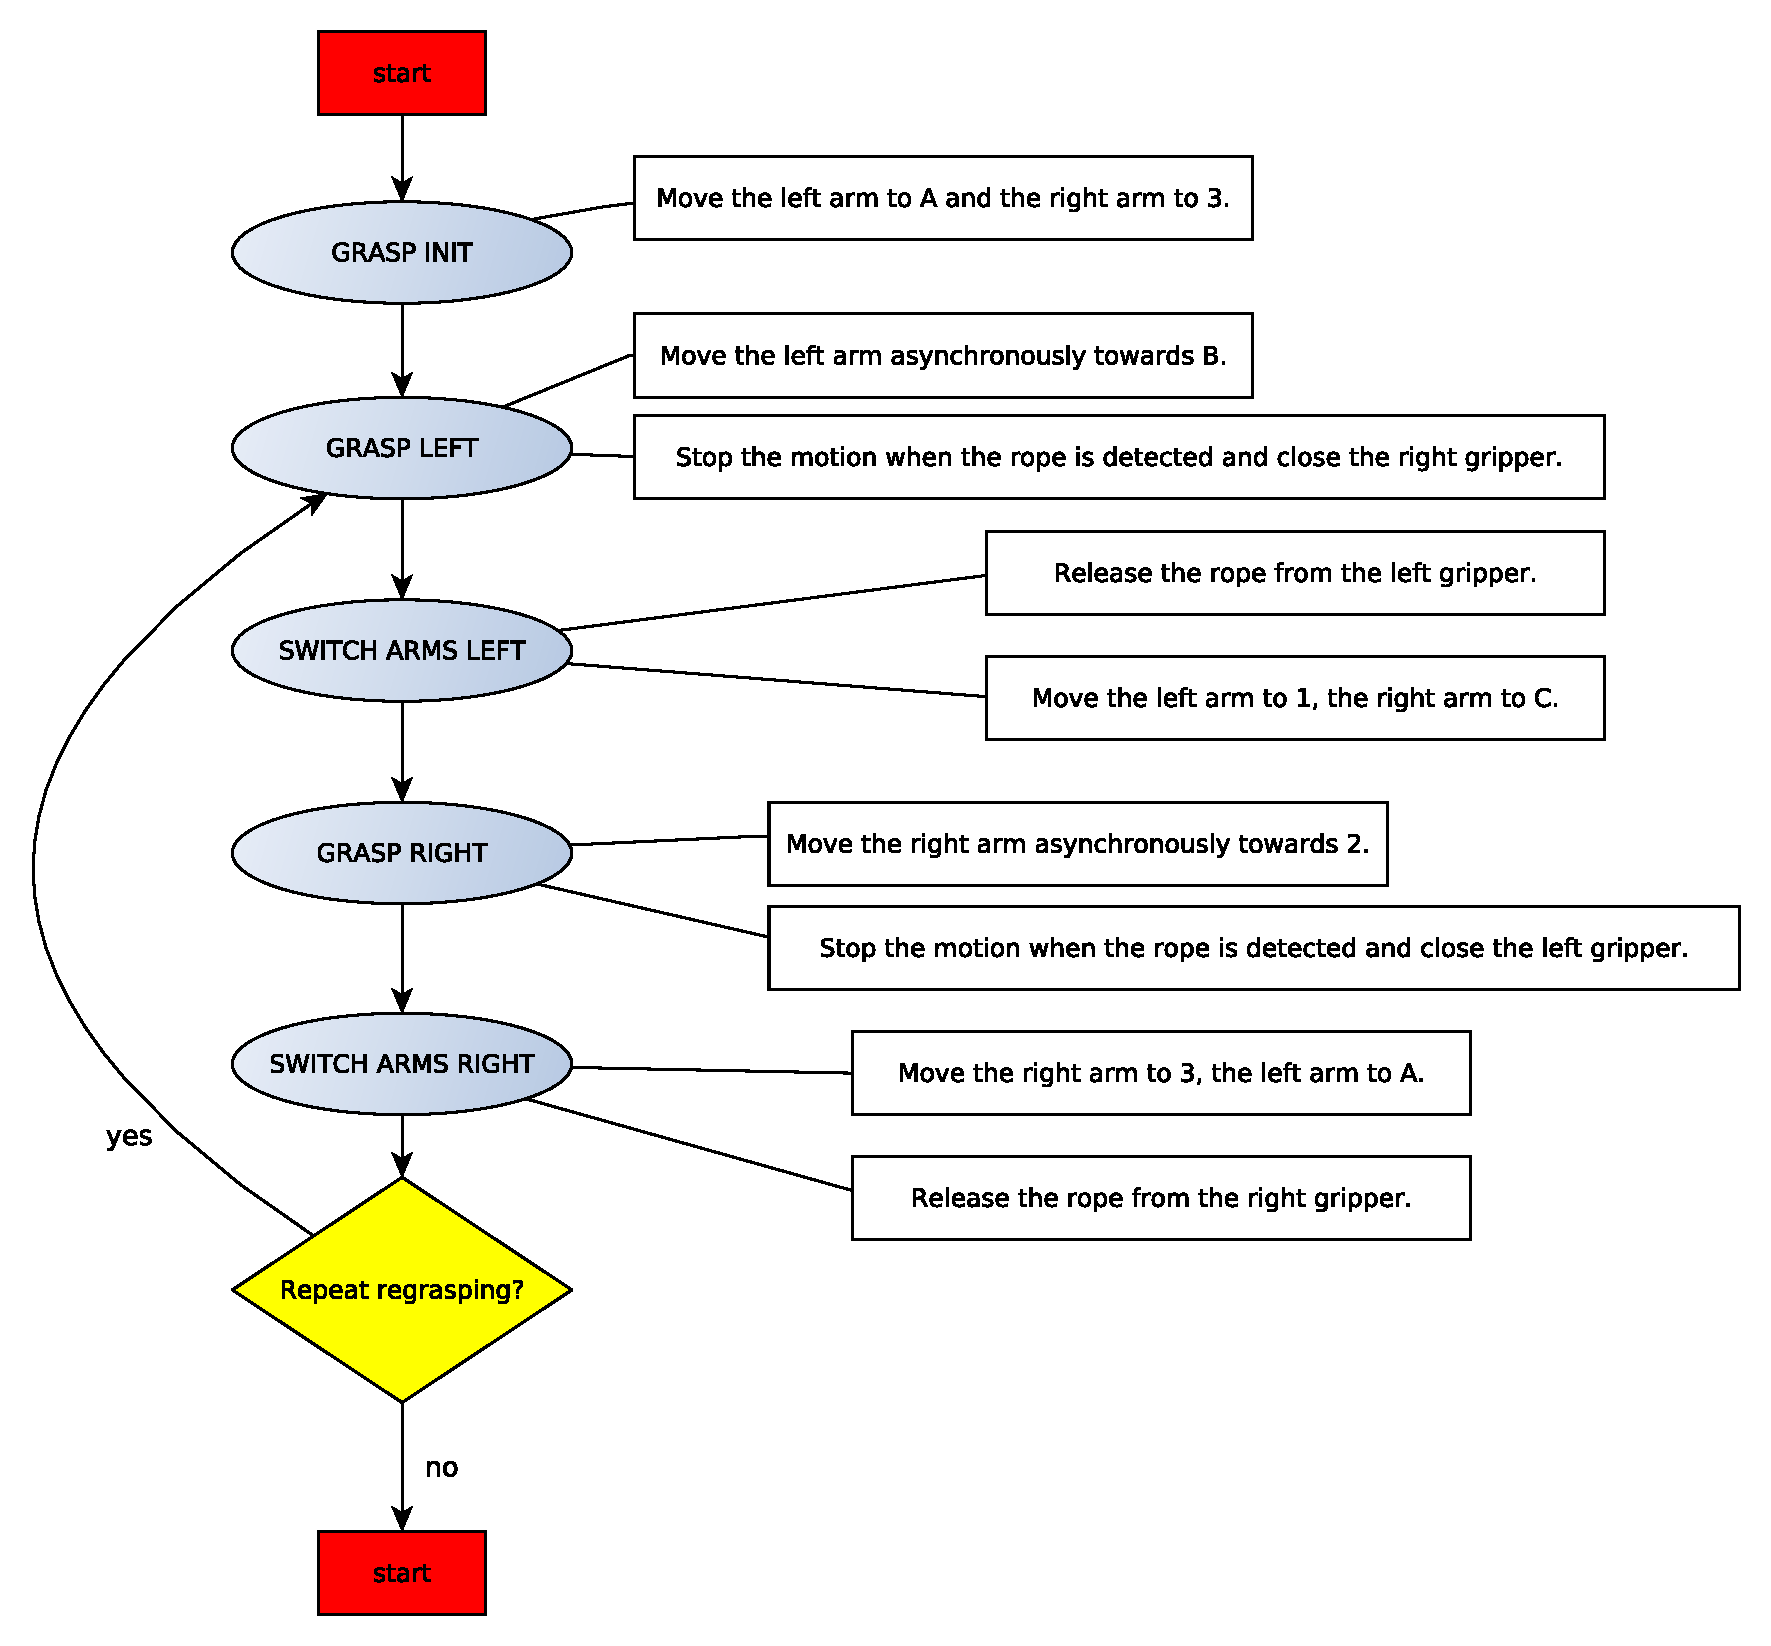
\includegraphics[width=1.0\textwidth]{RegraspingWorkflow.pdf}
        \centering
        \caption{The regrasping workflow.}
        \label{fig:RegraspingWorkflow}
        \end{figure}


        \begin{figure}
            \centering
            \begin{tabular}{c|c}
            \includegraphics[width=0.4\textwidth]{GraspLeft.pdf}
            %
            &
            %
            \includegraphics[width=0.4\textwidth]{SwitchLeft.pdf}
            \\
            1 & 2 \\
            \hline
            \includegraphics[width=0.4\textwidth]{GraspRight.pdf}
            %
            &
            %
            \includegraphics[width=0.4\textwidth]{SwitchRight.pdf} \\
            3 & 4 \\

            \end{tabular}
            \caption{1: Grasp left, 2: Switch arms left, 3: Grasp right, 4: Switch arms right.}
            \label{fig:RegraspingProcedure}
        \end{figure}

        \paragraph{GRASP INIT}~\\
            The left arm moves to point~$P_a$ and the right one to point~$P_3$. The right gripper holds the rope that is hanging down freely. The left gripper is fully opened and is positioned in such a way that the rope that is going to be moved towards it in the next step will enter the inside of the gripper (see Figure~\ref{fig:RegraspingProcedure},~1).

        \paragraph{GRASP LEFT}~\\
            The left arm starts moving slowly towards point~$P_b$. The rope thus enters the right gripper. As soon as the rope is detected (see Section~\ref{sec:DetectingTheRope}), the movement of the left arm is stopped and the right gripper closes, thus catching the rope (see Figure~\ref{fig:RegraspingProcedure}, 1).

        \paragraph{SWITCH ARMS LEFT}~\\
            First, the left gripper releases the upper end of the rope. It falls down, now hanging just from the right gripper. Second, the left arm moves to point~$P_c$ thus reaching a pose in which it will later be able to catch the moving rope. Finally, the right gripper turns by \SI{180}{\degree} to unwrap the rope from the gripper (see Figure~\ref{fig:RegraspingProcedure}, 2).

        \paragraph{GRASP RIGHT}~\\
            See \textbf{GRASP LEFT}, the function of both arms is swapped (see Figure~\ref{fig:RegraspingProcedure}, 3).

        \paragraph{SWITCH ARMS RIGHT}~\\
            See \textbf{SWITCH ARMS LEFT}, the function of both arms is swapped (see Figure~\ref{fig:RegraspingProcedure}, 4).

        The gripper rotates \SI{180}{\degree} around the $x$-axis upon transition from points $P_3$ to $P_1$ in the case of the right gripper and from $P_C$ to $P_A$ in the case of the left gripper. Let us know examine the case of the right gripper. The rope end that has fallen down from the left gripper might now be a bit ``wrapped'' around the right gripper (see Figure~\ref{fig:WrappedRopeCloseUp}). Therefore, the right gripper has to rotate to ensure that the rope gets ``unwrapped'' and can hang down freely.

        \begin{figure}[h]
        \includegraphics[width=0.3\textwidth]{WrappedRopeCloseUp.png}
        \centering
        \caption{The rope wrapped around the gripper.}
        \label{fig:WrappedRopeCloseUp}
        \end{figure}


    \subsection{Detecting the rope in the gripper} \label{sec:DetectingTheRope}

        The rope detection algorithm was originally tested on the rope R2 (white and twisted rope, see Table~\ref{table:AvailableRopes}). The left gripper holding the R2 rope was moved to point $P_b$ and the output of the proximity and light sensor placed in the right gripper was measured.

        I decided to use the proximity sensor over the light sensor for the rope detection, because the peak in the output of the proximity sensor was more distinct than the peak in the output of the light sensor (see Figure~\ref{fig:RopeDetection}, left side).

        The motion of the arm holding the rope is stopped, when a peak in the output of the proximity sensor passes. This approach proves more robust for ropes of different thicknesses (a thicker rope produces a higher peak) than a simple thresholding. However, a threshold is used to detect the rise of the peak. Initially, I set up the threshold to $r_0 = 100$ (see Figure~\ref{fig:RopeDetection}, right side). The threshold $r_0$ makes sure that the rope detection process does not react on noise in the output of the proximity sensor.


        \begin{figure}[h]
            \centering
            \begin{tabular}{cc}
            \includegraphics[width=0.49\textwidth]{ProximityVsLight.png}
            %
            &
            %
            \includegraphics[width=0.49\textwidth]{ProximityPeak.png}
            \end{tabular}
            \caption{Left: Comparing the proximity and light sensor. Right: Detecting the peak.}
            \label{fig:RopeDetection}
        \end{figure}


    \subsection{Experiments}
        I found out that the rope R2 is not suitable for the regrasping procedure. It did not become straight after it was regrasped, it was rather bent to one side. This behavior prevents the successful consecutive regrasping. For this reason, I decided to use a different rope (see Figure~\ref{fig:Regrasping}). To ensure that it becomes straight again, it has a weight on each end.

        I did not have to change the rope detection algorithm, it worked well for a thinner rope also. The only thing I had to adjust was to lower the threshold $r_0$ to 20, since the peak in the output of the proximity sensor became smaller.

        \begin{figure}
        \includegraphics[width=0.5\textwidth]{Regrasping.png}
        \centering
        \caption{The left arm regrasps the rope.}
        \label{fig:Regrasping}
        \end{figure}

        The procedure ran successfully for regrasping the rope from the right gripper to the left and back. It took \SI{34}{s}. The experiment was recorder on video that is called \textit{RegraspRope.mpg} and can be found on the attached CD.

    \subsection{Discussion}
        Although the robot managed to regrasp the rope successfully, a few additional features would have to be implemented in order to make the process continuous (i.e. to be able to regrasp the rope many times in a row). The point in which the upper gripper releases the rope should be moved a bit to the side. In this way, the rope would fall to a predictable side of the lower gripper. Thus, it would be possible to always unwrap the rope from the gripper by turning it by \SI{180}{\degree}. This does not happen in the present case, since the rope is released directly above the gripper and thus it is not predictable on which side of the gripper it falls down. 